%==================================================================
\frame{\frametitle{Super-motifs} \label{back:superMotifs}

  \begin{tabular}{ll}
    \begin{tabular}{p{.4\textwidth}}
      \paragraph{Motif:}
      $$
      \includegraphics[width=.1\textwidth, ]{\fignet/FigMotifsBEDD-motif9}
      $$
      ~\\ ~\\
      \paragraph{Variance:}
      $$
      \begin{array}{rcl}
        N_s^2 & = & \displaystyle{\left(\sum_\alpha Y_{s\alpha}\right)^2} \\
        ~ \\
        & = & \displaystyle{\sum_{\alpha, \beta: \alpha \cap \beta = \emptyset} Y_{s\alpha} Y_{s\beta}} \\
        ~ \\
        & & \displaystyle{+ \sum_{\alpha, \beta: \alpha \cap \beta \neq \emptyset} \underset{\footnotesize\begin{array}{c}\text{occurrence of} \\ \text{a super-motif} \end{array}}{\underbrace{Y_{s\alpha} Y_{s\beta}}}} \\
      \end{array}
      $$
    \end{tabular} 
    &
    \begin{tabular}{p{.5\textwidth}}
      \paragraph{Some super-motifs:} \\
      \includegraphics[width=.1\textwidth, ]{\fignet/FigMotifsBEDD-motif9-supermotif1} 
      \includegraphics[width=.1\textwidth, ]{\fignet/FigMotifsBEDD-motif9-supermotif2} 
      \includegraphics[width=.1\textwidth, ]{\fignet/FigMotifsBEDD-motif9-supermotif3} 
      \includegraphics[width=.1\textwidth, ]{\fignet/FigMotifsBEDD-motif9-supermotif4} \\
      \includegraphics[width=.1\textwidth, ]{\fignet/FigMotifsBEDD-motif9-supermotif5} 
      \includegraphics[width=.1\textwidth, ]{\fignet/FigMotifsBEDD-motif9-supermotif6} 
      \includegraphics[width=.1\textwidth, ]{\fignet/FigMotifsBEDD-motif9-supermotif7} 
      \includegraphics[width=.1\textwidth, ]{\fignet/FigMotifsBEDD-motif9-supermotif8} \\
      \includegraphics[width=.1\textwidth, ]{\fignet/FigMotifsBEDD-motif9-supermotif9} 
      \includegraphics[width=.1\textwidth, ]{\fignet/FigMotifsBEDD-motif9-supermotif10}
      \includegraphics[width=.1\textwidth, ]{\fignet/FigMotifsBEDD-motif9-supermotif11}
      \includegraphics[width=.1\textwidth, ]{\fignet/FigMotifsBEDD-motif9-supermotif12} \\
      \includegraphics[width=.1\textwidth, ]{\fignet/FigMotifsBEDD-motif9-supermotif13} 
      \includegraphics[width=.1\textwidth, ]{\fignet/FigMotifsBEDD-motif9-supermotif14}
      \includegraphics[width=.1\textwidth, ]{\fignet/FigMotifsBEDD-motif9-supermotif15}
      \includegraphics[width=.1\textwidth, ]{\fignet/FigMotifsBEDD-motif9-supermotif16} \\
      ~ \\
      \dots 396 super-motifs \\
      ~ \\ ~ \\ ~ \\ 
    \end{tabular} 
  \end{tabular}
  
  \paragraph{Covariance:} same game, for $Y_{s\alpha} Y_{s'\beta}$ with $s \neq s'$ \goto{sec:motifMoments}

}

%==================================================================
\frame{\frametitle{In practice: Asymptotic normality} \label{back:asymNormality}

  \begin{center}
    \begin{tabular}{cccc}
      ($n = 2m/3$) & $m=50$ & $m=100$ & $m=200$ \\
      \includegraphics[width=.1\textwidth]{\fignet/FigMotifsBEDD-adjMatMotif6} & 
      \includegraphics[width=.2\textwidth]{\fignet/FigMotifsBEDD-SimMotifBEDD-m50-n33-rho5-g2-h3-6nodesFALSE-B500-distCountMotif6} &
      \includegraphics[width=.2\textwidth]{\fignet/FigMotifsBEDD-SimMotifBEDD-m100-n67-rho5-g2-h3-6nodesFALSE-B500-distCountMotif6} &
      \includegraphics[width=.2\textwidth]{\fignet/FigMotifsBEDD-SimMotifBEDD-m200-n133-rho5-g2-h3-6nodesFALSE-B500-distCountMotif6} \\
      \includegraphics[width=.1\textwidth]{\fignet/FigMotifsBEDD-adjMatMotif16} & 
      \includegraphics[width=.2\textwidth]{\fignet/FigMotifsBEDD-SimMotifBEDD-m50-n33-rho5-g2-h3-6nodesFALSE-B500-distCountMotif16} &
      \includegraphics[width=.2\textwidth]{\fignet/FigMotifsBEDD-SimMotifBEDD-m100-n67-rho5-g2-h3-6nodesFALSE-B500-distCountMotif16} &
      \includegraphics[width=.2\textwidth]{\fignet/FigMotifsBEDD-SimMotifBEDD-m200-n133-rho5-g2-h3-6nodesFALSE-B500-distCountMotif16} \\
    \end{tabular}
  \end{center}
  
  \bigskip
  \textcolor{blue}{Normal} distribution, \textcolor{magenta}{Poisson-geometric} distribution with same mean and variance \refer{Sta01,PDK08} \goto{sec:motifMoments}


}

%==================================================================
\frame{\frametitle{In practice: Test statistic} \label{back:motifTest}

  \paragraph{Need to account for the estimation error} of $\widehat{\Esp} N$
  
  \begin{center}
  \begin{tabular}{lccc}
    & $m=50$ & $m=100$ & $m=200$ \\
    \begin{tabular}{p{.175\textwidth}}
    Regular stat.: 
    $$
    {\frac{N - \widehat{\Esp} N}{\sqrt{\widehat{\Var} N}}}
    $$
    \end{tabular}
    & 
    \begin{tabular}{c}
    \includegraphics[width=.2\textwidth]{\fignet/FigMotifsBEDD-SimMotifBEDD-m50-n33-rho5-g2-h3-6nodesFALSE-B500-distRawStat6}
    \end{tabular}
    & 
    \begin{tabular}{c}
    \includegraphics[width=.2\textwidth]{\fignet/FigMotifsBEDD-SimMotifBEDD-m100-n67-rho5-g2-h3-6nodesFALSE-B500-distRawStat6}
    \end{tabular}
    & 
    \begin{tabular}{c}
    \includegraphics[width=.2\textwidth]{\fignet/FigMotifsBEDD-SimMotifBEDD-m200-n133-rho5-g2-h3-6nodesFALSE-B500-distRawStat6}
    \end{tabular}
    \\ \pause
    \begin{tabular}{p{.175\textwidth}}
    Correction: 
    $$
    {\frac{N - (\widehat{\Esp} N - \emphase{\widehat{\Bias}(\widehat{\Esp} N)})}{\sqrt{\emphase{\widehat{\Var} (N - \widehat{\Esp} N)}}}}
    $$
    \end{tabular}
    & 
    \begin{tabular}{c}    
    \includegraphics[width=.2\textwidth]{\fignet/FigMotifsBEDD-SimMotifBEDD-m50-n33-rho5-g2-h3-6nodesFALSE-B500-distNormStat6}
    \end{tabular}
    & 
    \begin{tabular}{c}
    \includegraphics[width=.2\textwidth]{\fignet/FigMotifsBEDD-SimMotifBEDD-m100-n67-rho5-g2-h3-6nodesFALSE-B500-distNormStat6}
    \end{tabular}
    & 
    \begin{tabular}{c}    
    \includegraphics[width=.2\textwidth]{\fignet/FigMotifsBEDD-SimMotifBEDD-m200-n133-rho5-g2-h3-6nodesFALSE-B500-distNormStat6}
    \end{tabular}
  \end{tabular}
  \end{center}
  
  \begin{itemize}
    \item Need to evaluate \emphase{$\Var(N - \widehat{\Esp}(N))$} and \emphase{$\Bias(\widehat{\Esp} N)$}: resort to Taylor expansion ($\Delta-$method) \goto{sec:GOF}
  \end{itemize}
}

%==================================================================
\frame{\frametitle{Choleski transform} \label{back:cholesky}

  \bigskip
  \paragraph{Aim:} 'Remove' correlation and variance heterogeneity 
  
  \bigskip
  \begin{tabular}{cc}
    \hspace{-0.04\textwidth}
    \begin{tabular}{p{.45\textwidth}}
      \paragraph{Covariance matrix of $(X_1, X_2)$:}
      $$
      \Sigma_{X_1, X_2} = \left[\begin{array}{cc} 
                      \sigma^2_1 & \sigma_{12} \\
                      \sigma_{12} & \sigma^2_2 \\
                     \end{array}\right]
      $$
    \end{tabular}
    & 
    \begin{tabular}{p{.45\textwidth}}
      \onslide+<2->{\paragraph{Choleski transform:}
      $$
      \left[\begin{array}{c} X'_1 \\ X'_2 \end{array} \right]
      = \Sigma^{-1/2} \left[\begin{array}{c} X_1 \\ X_2 \end{array} \right]
      $$}
    \end{tabular} 
    \\
    \hspace{-0.04\textwidth}
    \begin{tabular}{c}
      \vspace{-0.08\textheight}
      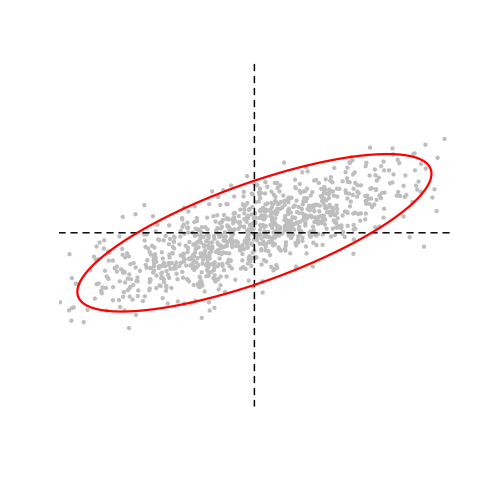
\includegraphics[width=0.35\textwidth, trim=25 25 25 25, clip=]{\fignet/Cholevski-raw} 
    \end{tabular}
    & 
    \begin{tabular}{c}
      \vspace{-0.08\textheight}
      \onslide+<2->{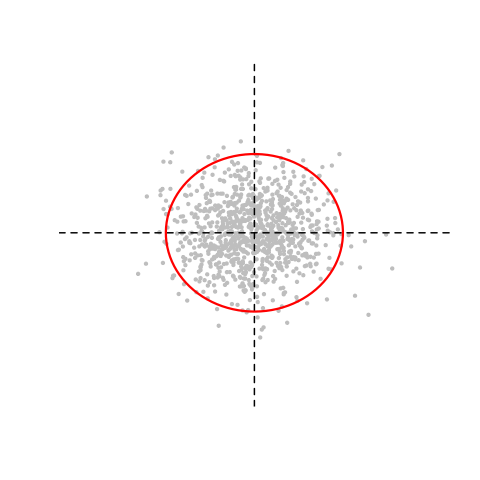
\includegraphics[width=0.35\textwidth, trim=25 25 25 25, clip=]{\fignet/Cholevski-chol}}
    \end{tabular} 
    \\
    \hspace{-0.04\textwidth}
    \begin{tabular}{p{.45\textwidth}}
      Diagonalization: $\Sigma = P \emphase{\Lambda} P^{-1}$ \\
      ~ \\
      Choleski matrix: $\Sigma^{-1/2} = P \emphase{\Lambda^{-1/2}} P^{-1}$
    \end{tabular}
    & \pause
    \begin{tabular}{p{.45\textwidth}}
      \onslide+<2->{$$
      \Sigma_{X'_1, X'_2} = \left[\begin{array}{cc} 
                      1 & 0 \\
                      0 & 1 \\
                     \end{array}\right]
      $$
      \goto{sec:cholesky}
      }
    \end{tabular} 
  \end{tabular}

}

%==================================================================
%==================================================================
\section{Network embedding}
\frame{\frametitle{Outline} \tableofcontents[currentsection]}
%==================================================================
\frame{\frametitle{Network embedding: Multivariate analysis}

  \paragraph{Analysing multiple networks.} Principle
  \begin{itemize}
   \item 'Embed' each network into a convenient space (e.g. $\Rbb^d$)
   \item Use standard multivariate analysis (clustering, PCA, MDS, ...)
  \end{itemize}
  
  \bigskip \bigskip \pause
  \paragraph{Using motifs.} $K$ networks 
  $$
  (\text{Network})_k \quad \rightarrow \quad
  (N^k_1, \dots, N^k_S) \in \Rbb^S
  $$
  but need to correct for: network sizes, correlation between motif frequencies, etc...

  \bigskip \bigskip \pause
  \hspace{-.05\textwidth}
  \begin{tabular}{ll}
    \begin{tabular}{p{.4\textwidth}}
      \paragraph{~Zackenberg dataset.} $K = 46$ networks 
      \begin{itemize}
      \item 2 years
      \item 1 network observed every few days 
      \end{itemize}
    \end{tabular}
    &
    \begin{tabular}{p{.5\textwidth}}
      \includegraphics[width=.1\textwidth]{\fignet/Zackenberg-red-96:5-adj}
      \includegraphics[width=.1\textwidth]{\fignet/Zackenberg-red-96:10-adj}
      \includegraphics[width=.1\textwidth]{\fignet/Zackenberg-red-96:15-adj} 
      \includegraphics[width=.1\textwidth]{\fignet/Zackenberg-red-96:20-adj} 
      \dots \\
      \includegraphics[width=.1\textwidth]{\fignet/Zackenberg-red-97:5-adj}
      \includegraphics[width=.1\textwidth]{\fignet/Zackenberg-red-97:10-adj}
      \includegraphics[width=.1\textwidth]{\fignet/Zackenberg-red-97:15-adj} 
      \includegraphics[width=.1\textwidth]{\fignet/Zackenberg-red-97:20-adj} 
      \dots
    \end{tabular} 
  \end{tabular}

}

%==================================================================
\frame{\frametitle{Network embedding: Zackenberg's data \refer{SRO16}} \label{sec:cholesky}

  \bigskip
  \begin{tabular}{c|c|c|c}
    \onslide+<1->{Raw counts} & 
    \onslide+<2->{Corrected stat.} & 
    \onslide+<3->{Choleski \goto{back:cholesky}.} & 
    \onslide+<4>{Bray-Curtis MDS} \\
    \hline
    \onslide+<1->{\includegraphics[width=.2\textwidth, height=.175\textheight]{\fignet/Zackenberg-red-PCAcount-scree}} &
    \onslide+<2->{\includegraphics[width=.2\textwidth, height=.175\textheight]{\fignet/Zackenberg-red-PCAstat-scree}} & 
    \onslide+<3->{\includegraphics[width=.2\textwidth, height=.175\textheight]{\fignet/Zackenberg-red-PCAchol-scree}} &  
    \onslide+<4>{\includegraphics[width=.2\textwidth, height=.175\textheight]{\fignet/Zackenberg-red-MDSBrayCurtis-scree}}
    \\
    \onslide+<1->{\includegraphics[width=.22\textwidth]{\fignet/Zackenberg-red-PCAcount-biplot}} &
    \onslide+<2->{\includegraphics[width=.22\textwidth]{\fignet/Zackenberg-red-PCAstat-biplot}} &
    \onslide+<3->{\includegraphics[width=.22\textwidth]{\fignet/Zackenberg-red-PCAchol-biplot}} &
    \onslide+<4>{\includegraphics[width=.22\textwidth]{\fignet/Zackenberg-red-MDSBrayCurtis-biplot}}
    \\
    \onslide+<1->{\includegraphics[width=.2\textwidth]{\fignet/Zackenberg-red-PCAcount-size}} &
    \onslide+<2->{\includegraphics[width=.2\textwidth]{\fignet/Zackenberg-red-PCAstat-size}} &
    \onslide+<3->{\includegraphics[width=.2\textwidth]{\fignet/Zackenberg-red-PCAchol-size}} &
    \onslide+<4>{\includegraphics[width=.2\textwidth]{\fignet/Zackenberg-red-MDSBrayCurtis-size}}
  \end{tabular}

}

%==================================================================
\frame{\frametitle{Goodness-of-fit (GOF) of the BEDD model} \label{back:GOF}

  \hspace{-.05\textwidth}
  \begin{tabular}{ll}
    \begin{tabular}{p{.5\textwidth}}
      \onslide+<1->{\paragraph{Raw statistic:}
      $$
      T_s = \frac{N_s - \widehat{\Esp} N_s}{\sqrt{\widehat{\Var} N_s}}
      $$ \\ 
      }
      \onslide+<2->{
      \paragraph{Corrected stat.:} accounts for the estimation error in $\widehat{\Esp} N$
      $$
      T'_s = \frac{N_s - (\widehat{\Esp} N_s - \emphase{\widehat{\Bias}(\widehat{\Esp} N_s)})}{\sqrt{\emphase{\widehat{\Var} (N_s - \widehat{\Esp} N_s)}}}
      $$ \\ 
      }
      \onslide+<3>{\paragraph{Cholevski      
      \footnote{$\Sigma = P \Lambda P^\intercal$, $\Sigma = P \Lambda^{-1/2} P^\intercal$} 
      transformation:} accounts for the correlation between the counts
      $$
      \Sigma_{s, s'} = \Cov(N_s - \widehat{\Esp} N_s, N_{s'} - \widehat{\Esp} N_{s'})
      $$
      $$
      T'' = \emphase{\widehat{\Sigma}^{-1/2}}
      \left[N_s - (\widehat{\Esp} N_s - \widehat{\Bias}(\widehat{\Esp} N_s))\right]
      $$
      }
    \end{tabular}
    &
    \begin{tabular}{p{.4\textwidth}}
      \hspace{-.05\textwidth}
      \onslide+<1->{\paragraph{Zackenberg network.} ~ \\}
      \begin{overprint}
        \onslide<1>
        \includegraphics[width=.4\textwidth]{\fignet/Zackenberg-1996_12-red-StatCount}
        \onslide<2>
        \includegraphics[width=.4\textwidth]{\fignet/Zackenberg-1996_12-red-NormStatCount}
        \onslide<3>
        \includegraphics[width=.4\textwidth]{\fignet/Zackenberg-1996_12-red-CholNormStat}
      \end{overprint}
      \goto{sec:GOF}
    \end{tabular} 
  \end{tabular}

}


%==================================================================
\frame{\frametitle{An intuition for Adonis} \label{back:adonis} 

  \bigskip
  \paragraph{Variance.} Remind that
  $
  \displaystyle{\sum_{i=1}^n (y_i - \overline{y})^2 = \frac1{2n} \sum_{i=1}^n \sum_{i'=1}^n (y_i - y_{i'})^2}
  $

  \bigskip \pause
  \paragraph{Analysis of variance.} Remind that, for $g$ groups, with $r$ replicates ($n = r \; g$), 
  \begin{align*}
  \underset{\text{\normalsize{Total}}}{\underbrace{\sum_{i=1}^g \sum_{j=1}^r (y_{ij} - \overline{y})^2}}
  & =
  \underset{\text{\normalsize{Between}}}{\underbrace{\sum_{i=1}^g r \; (\overline{y}_i - \overline{\overline{y}})^2}}
  +
  \underset{\text{\normalsize{Within}}}{\underbrace{\sum_{i=1}^g \sum_{j=1}^r (y_{ij} - \overline{y}_i)^2}} \\
  \text{Anova test statistic} \quad  \emphase{F} & \emphase{\propto \text{Between}/\text{Within}}
  \end{align*} 

  \bigskip \pause
  \paragraph{Distance.} $p$ variables $y_{ij} = (y_{ijk})_{k = 1 \dots p}$:
  $
  \displaystyle{D^2(y_{ij}, y_{i'j'}) = \sum_{k=1}^p (y_{ijk} - y_{i'j'k})^2}
  $

  \bigskip \pause
  \paragraph{Adonis.} Define Between = Total - Within, where
  \begin{align*}
    \text{Total} 
    & = \frac1{2n} \sum_{i=1}^g \sum_{i'=1}^g \sum_{j'=1}^r D^2(y_{ij}, y_{i'j'}), &
    \text{Within} 
    & = \frac1{2} \sum_{i=1}^g  \sum_{j=1}^r \sum_{j'=1}^r D^2(y_{ij}, y_{i'j'}), &
  \end{align*}
  and determine the $p$-value for $F = \text{Between}/\text{Within}$ by permutation. 
  \goto{sec:adonis}
  
}

%==================================================================
\frame{\frametitle{Null simulations} \label{back:adonisNull} 

  100 sets of $83$ synthetic networks, with dimensions as the original ones and fixed $\rho$, $g$, and $h$

  \bigskip
  \begin{tabular}{lc|cl}
%     \hspace{-.05\textwidth}
    \paragraph{Without correction.} & & & \paragraph{Over 100 networks.} \\
    \begin{tabular}{p{.5\textwidth}}
%       \paragraph{Without correction.} \\
      \tiny{\begin{tabular}{l|rrrrr}
         & Df & SumOfSqs & $R^2$ & F & Pr(\>F) \\ 
\hline
Year & 1 & 1.5 & 0.0114 & 0.94 & 0.443 \\ 
Month & 6 & 25.17 & 0.1914 & 2.61 & \emphase{0.012} \\ 
Region & 2 & 0.69 & 0.0052 & 0.21 & 0.845 \\ 
Year:Month & 6 & 7.46 & 0.0568 & 0.77 & 0.653 \\ 
Year:Region & 2 & 2.52 & 0.0191 & 0.78 & 0.543 \\ 
Month:Region & 12 & 12.55 & 0.0954 & 0.65 & 0.831 \\ 
Year:Month:Region & 12 & 17.39 & 0.1322 & 0.9 & 0.578 \\ 
Residual & 40 & 64.23 & 0.4884 & & \\ 
Total & 81 & 131.51 & 1 & &

      \end{tabular}}
    \end{tabular}
    & \quad & \quad & 
    \begin{tabular}{p{.35\textwidth}}
%       \paragraph{Over 100 networks.} \\
      \includegraphics[width=.25\textwidth, trim=10 10 10 40, clip=]{\fignatB/AdonisCorrection-stat1-adonis1-2-Month-permut9999-boxplot}
    \end{tabular} 
    \\
    & & & 
    \\
    \paragraph{With correction.} & & & \paragraph{Increasing the networks' size.} \\
%     \hspace{-.05\textwidth}
    \begin{tabular}{p{.45\textwidth}}
%       \paragraph{With correction.} \\
      \tiny{\begin{tabular}{l|rrrrr}
         & Df & SumOfSqs & $R^2$ & F & Pr(\>F) \\ 
 \hline
insectNb & 1 & 10.55 & 0.0803 & 7.17 & \emphase{0.003} \\ 
plantNb & 1 & 7.32 & 0.0556 & 4.97 & \emphase{0.015} \\ 
Year & 1 & 0.77 & 0.0059 & 0.53 & 0.622 \\ 
Month & 6 & 8.96 & 0.0681 & 1.01 & 0.458 \\ 
Region & 2 & 4.39 & 0.0334 & 1.49 & 0.241 \\ 
Year:Month & 6 & 8.54 & 0.0649 & 0.97 & 0.496 \\ 
Year:Region & 2 & 2.17 & 0.0165 & 0.74 & 0.569 \\ 
Month:Region & 12 & 13.99 & 0.1064 & 0.79 & 0.699 \\ 
Year:Month:Region & 12 & 18.9 & 0.1437 & 1.07 & 0.421 \\ 
Residual & 38 & 55.93 & 0.4253 & & \\ 
Total & 81 & 131.51 & 1 & &

      \end{tabular}} \\
      \goto{sec:adonisResults}
    \end{tabular}
    & \quad & \quad & 
    \begin{tabular}{p{.35\textwidth}}
%       \paragraph{Increasing the networks' size.} \\
      \includegraphics[width=.25\textwidth, trim=10 10 10 40, clip=]{\fignatB/EffectNetworkSize-stat1-adonis1-Month-permut9999-boxplot}
    \end{tabular} 
  \end{tabular}

}

%==================================================================
\frame{\frametitle{Results for other motif distances} \label{back:adonisOther}

  \paragraph{Plant imbalance $D^{(h)}$.}
  $$\footnotesize{
  \begin{tabular}{l|rrrrr}
    & Df & Sum Of Sqs & $R^2$ & F & Pr(\>F) \\ 
 \hline
\textcolor{red}{\bf insectNb} & 1 & 9.81 & 0.1935 & 19.53 & \textcolor{red}{\bf 1e-05} \\ 
{\bf plantNb} & 1 & 1.42 & 0.028 & 2.83 & {\bf 0.06594} \\ 
Year & 1 & 0.67 & 0.0133 & 1.34 & 0.27518 \\ 
Month & 6 & 4.14 & 0.0818 & 1.38 & 0.20713 \\ 
Region & 2 & 0.99 & 0.0196 & 0.99 & 0.43126 \\ 
Year:Month & 6 & 2.61 & 0.0514 & 0.86 & 0.58258 \\ 
Year:Region & 2 & 1.87 & 0.037 & 1.87 & 0.1283 \\ 
Month:Region & 12 & 4.33 & 0.0854 & 0.72 & 0.8062 \\ 
Year:Month:Region & 12 & 5.75 & 0.1135 & 0.95 & 0.53039 \\ 
Residual & 38 & 19.09 & 0.3766 & & \\ 
Total & 81 & 50.69 & 1 & & \\ 

  \end{tabular}
  }$$

  \paragraph{Both imbalance $D^{(gh)}$.}
  $$\footnotesize{
  \begin{tabular}{l|rrrrr}
    & Df & Sum Of Sqs & $R^2$ & F & Pr(\>F) \\ 
 \hline
\textcolor{red}{\bf insectNb} & 1 & 56.21 & 0.265 & 48.58 & \textcolor{red}{\bf 1e-05} \\ 
\textcolor{red}{\bf plantNb} & 1 & 16.44 & 0.0775 & 14.21 & \textcolor{red}{\bf 1e-05} \\ 
Year & 1 & 0.83 & 0.0039 & 0.71 & 0.56559 \\ 
\textcolor{red}{\bf Month} & 6 & 24.41 & 0.1151 & 3.52 & \textcolor{red}{\bf 0.00012} \\ 
\textcolor{red}{\bf Region} & 2 & 8.83 & 0.0417 & 3.82 & \textcolor{red}{\bf 0.00321} \\ 
Year:Month & 6 & 10.09 & 0.0476 & 1.45 & 0.14299 \\ 
Year:Region & 2 & 3.15 & 0.0149 & 1.36 & 0.25071 \\ 
\textcolor{red}{\bf Month:Region} & 12 & 29.92 & 0.1411 & 2.16 & \textcolor{red}{\bf 0.0028} \\ 
Year:Month:Region & 12 & 18.24 & 0.086 & 1.31 & 0.16496 \\ 
Residual & 38 & 43.96 & 0.2073 & & \\ 
Total & 81 & 212.09 & 1 & & 

  \end{tabular}
  }$$
  \goto{sec:adonisResults}

}

